\documentclass{article}
\usepackage[utf8]{inputenc}
\usepackage{graphicx}

\begin{document}
\title{Day 1}

\author{\emph{Teemu Sarapisto}}
\maketitle

\newpage
\section{Original, noisy and filtered images}
\newcommand{\aaa}[3]{%
  \fbox{\includegraphics[height=30mm]{#1}} \quad
  \fbox{\includegraphics[height=30mm]{#2}} \quad
  \fbox{\includegraphics[height=30mm]{#3}} \par}

\newcommand{\bbb}[3]{%
  \medskip\noindent\aaa{#1}{#1-#2}{#1-#3}}

\setlength{\fboxsep}{0pt}%

pattern low pass

\bbb{p}{l3}{l5}
\bbb{p-ga1}{l3}{l5}
\bbb{p-ga2}{l3}{l5}
\bbb{p-sp1}{l3}{l5}
\bbb{p-sp2}{l3}{l5}

\pagebreak

messi low pass

\bbb{m}{l3}{l5}
\bbb{m-ga1}{l3}{l5}
\bbb{m-ga2}{l3}{l5}
\bbb{m-sp1}{l3}{l5}
\bbb{m-sp2}{l3}{l5}

\pagebreak

pattern median

\bbb{p}{m3}{m5}
\bbb{p-ga1}{m3}{m5}
\bbb{p-ga2}{m3}{m5}
\bbb{p-sp1}{m3}{m5}
\bbb{p-sp2}{m3}{m5}

\pagebreak

messi median

\bbb{m}{m3}{m5}
\bbb{m-ga1}{m3}{m5}
\bbb{m-ga2}{m3}{m5}
\bbb{m-sp1}{m3}{m5}
\bbb{m-sp2}{m3}{m5}

\pagebreak

pattern high pass

\bbb{p}{h3}{h5}
\bbb{p-ga1}{h3}{h5}
\bbb{p-ga2}{h3}{h5}
\bbb{p-sp1}{h3}{h5}
\bbb{p-sp2}{h3}{h5}

\pagebreak

messi high pass

\bbb{m}{h3}{h5}
\bbb{m-ga1}{h3}{h5}
\bbb{m-ga2}{h3}{h5}
\bbb{m-sp1}{h3}{h5}
\bbb{m-sp2}{h3}{h5}

\pagebreak

\section{}
 \subsection{Analyse what happened to pattern image and the messi images in all filterings and compare the properties of low-pass and median filerings}

 Low-pass "smudged" the image in both cases, was able to remove a little bit of noise. The pattern was quickly erased by it. Median smoothed out things, and was especially good at removing noise. High-pass brought out the edges in both pattern and messi image, but didn't remove any noise.

 Low pass resulted in more noisy and smudgy images compared to median. Median keeped it smoother, and was able get much better results for removing high amounts of salt\&pepper noise.

 \subsection{Finally, perform OpenCV’s histogram equalization to the original messi image and show also the histograms before and after equalization}
  \fbox{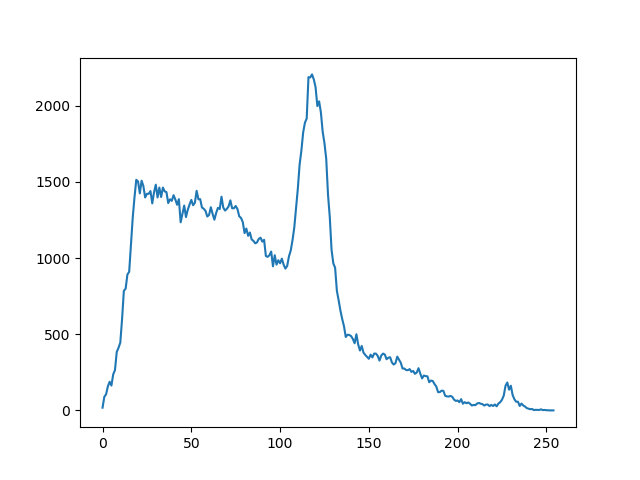
\includegraphics[height=50mm]{messi_hist_before} \par}
  \fbox{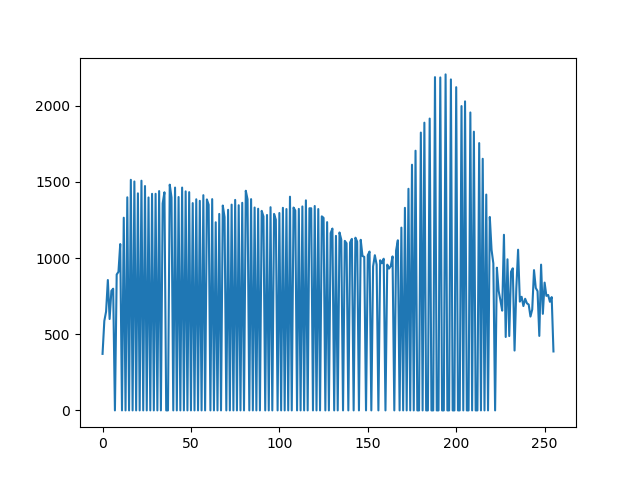
\includegraphics[height=50mm]{messi_hist_after} \par}
  \fbox{\includegraphics[height=50mm]{m} \par}
  \fbox{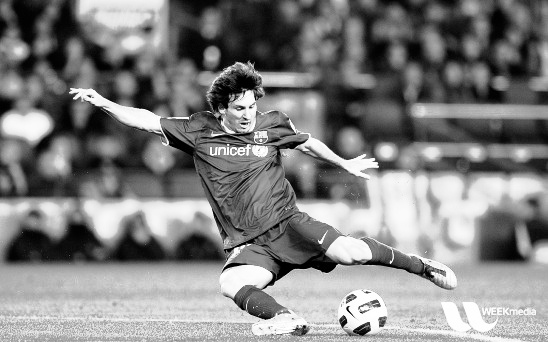
\includegraphics[height=50mm]{messi_after_hist} \par}

 \subsection{Report also, how long it took for you to complete the hands-on exercise}
    5 - 6 hours

    \section{Code used}
\begin{verbatim}
    #! /usr/bin/env python3

# https://docs.opencv.org/3.1.0/d6/d00/tutorial_py_root.html
# https://github.com/abidrahmank/OpenCV2-Python-Tutorials

import cv2
import numpy as np
import matplotlib.pyplot as plt
from scipy import ndimage as nd


def random_gauss(A, r):
    return np.random.normal(0, r, A.shape)

def clip(i):
    return np.clip(i, 0, 1)

p = cv2.imread('pattern.pbm', cv2.IMREAD_GRAYSCALE) / 255
m = cv2.imread('messi-gray.tiff', cv2.IMREAD_GRAYSCALE) / 255

p_ga1 = clip(p + random_gauss(p, 0.05))
p_ga2 = clip(p + random_gauss(p, 0.15))

### Tehtävä 5
gaussed_m1 = clip(m + random_gauss(m, 0.05))
gaussed_m2 = clip(m + random_gauss(m, 0.15))

### Tehtävä 6
def random_saltpepper(A, r):
    B = A + np.random.binomial(1, r/2, A.shape) # pepper
    C = B * np.random.binomial(1, 1 - (r/2), A.shape) # salt
    return C

### Tehtävä 7
pattern_peppered1 = clip(random_saltpepper(p, 0.1))
pattern_peppered2 = clip(random_saltpepper(p, 0.5))
m_peppered1 = clip(random_saltpepper(m, 0.1))
m_peppered2 = clip(random_saltpepper(m, 0.5))

### Tehtävä 8
def lowpass(A, n):
    weights = [[1 for x in range(n)] for y in range(n)]
    return nd.filters.convolve(A, weights) / (n*n)

### Tehtävä 9

pattern_lp1 = lowpass(p, 3)
pattern_lp2 = lowpass(p, 5)
gaussed_pattern1_lp1 = lowpass(p_ga1, 3)
gaussed_pattern1_lp2 = lowpass(p_ga1, 5)
gaussed_pattern2_lp1 = lowpass(p_ga2, 3)
gaussed_pattern2_lp2 = lowpass(p_ga2, 5)
pattern_peppered1_lp1 = lowpass(pattern_peppered1, 3) 
pattern_peppered1_lp2 = lowpass(pattern_peppered1, 5) 
pattern_peppered2_lp1 = lowpass(pattern_peppered2, 3) 
pattern_peppered2_lp2 = lowpass(pattern_peppered2, 5) 


m_lp1 = lowpass(m, 3)
m_lp2 = lowpass(m, 5)
gaussed_m1_lp1 = lowpass(gaussed_m1, 3)
gaussed_m1_lp2 = lowpass(gaussed_m1, 5)
gaussed_m2_lp1 = lowpass(gaussed_m2, 3)
gaussed_m2_lp2 = lowpass(gaussed_m2, 5)
m_peppered1_lp1 = lowpass(m_peppered1, 3) 
m_peppered1_lp2 = lowpass(m_peppered1, 5) 
m_peppered2_lp1 = lowpass(m_peppered2, 3) 
m_peppered2_lp2 = lowpass(m_peppered2, 5) 

# Tehtävä 10
def highpass(A, n):
    w = 25
    weights = [[(-1) for x in range(n)] for y in range(n)]
    x = int(n/2)
    y = int(n/2)
    weights[x][y] = w 
    return nd.filters.convolve(A, weights) / (n*n)


### Tehtävä 11
pattern_hp1 = clip(highpass(p, 3) + 0.5)
pattern_hp2 = clip(highpass(p, 5) + 0.5)
gaussed_pattern1_hp1 = clip(highpass(p_ga1, 3) + 0.5)
gaussed_pattern1_hp2 = clip(highpass(p_ga1, 5) + 0.5)
gaussed_pattern2_hp1 = clip(highpass(p_ga2, 3) + 0.5)
gaussed_pattern2_hp2 = clip(highpass(p_ga2, 5) + 0.5)
pattern_peppered1_hp1 = clip(highpass(pattern_peppered1, 3) + 0.5)
pattern_peppered1_hp2 = clip(highpass(pattern_peppered1, 5) + 0.5)
pattern_peppered2_hp1 = clip(highpass(pattern_peppered2, 3) + 0.5)
pattern_peppered2_hp2 = clip(highpass(pattern_peppered2, 5) + 0.5)

m_hp1 = clip(highpass(m, 3) + 0.5)
m_hp2 = clip(highpass(m, 5) + 0.5)
gaussed_m1_hp1 = clip(highpass(gaussed_m1, 3) + 0.5)
gaussed_m1_hp2 = clip(highpass(gaussed_m1, 5) + 0.5)
gaussed_m2_hp1 = clip(highpass(gaussed_m2, 3) + 0.5)
gaussed_m2_hp2 = clip(highpass(gaussed_m2, 5) + 0.5)
m_peppered1_hp1 = clip(highpass(m_peppered1, 3) + 0.5)
m_peppered1_hp2 = clip(highpass(m_peppered1, 5) + 0.5)
m_peppered2_hp1 = clip(highpass(m_peppered2, 3) + 0.5) 
m_peppered2_hp2 = clip(highpass(m_peppered2, 5) + 0.5) 

### Tehtävä 12
def median(A, n):
    return nd.filters.median_filter(A, n)

### Tehtävä 13
pattern_md1 = median(p, 3)
pattern_md2 = median(p, 5)
gaussed_pattern1_md1 = median(p_ga1, 3)
gaussed_pattern1_md2 = median(p_ga1, 5)
gaussed_pattern2_md1 = median(p_ga2, 3)
gaussed_pattern2_md2 = median(p_ga2, 5)
pattern_peppered1_md1 = median(pattern_peppered1, 3) 
pattern_peppered1_md2 = median(pattern_peppered1, 5) 
pattern_peppered2_md1 = median(pattern_peppered2, 3) 
pattern_peppered2_md2 = median(pattern_peppered2, 5) 

m_md1 = median(m, 3)
m_md2 = median(m, 5)
gaussed_m1_md1 = median(gaussed_m1, 3)
gaussed_m1_md2 = median(gaussed_m1, 5)
gaussed_m2_md1 = median(gaussed_m2, 3)
gaussed_m2_md2 = median(gaussed_m2, 5)
m_peppered1_md1 = median(m_peppered1, 3) 
m_peppered1_md2 = median(m_peppered1, 5) 
m_peppered2_md1 = median(m_peppered2, 3) 
m_peppered2_md2 = median(m_peppered2, 5) 

### Tehtävä 14
cv2.imwrite('p.jpg', cv2.resize(p * 255, None, fx=20, fy=20, interpolation=cv2.INTER_AREA))
cv2.imwrite('p-ga1.jpg', cv2.resize(p_ga1 * 255, None, fx=20, fy=20, interpolation=cv2.INTER_AREA))
cv2.imwrite('p-ga2.jpg', cv2.resize(p_ga2 * 255, None, fx=20, fy=20, interpolation=cv2.INTER_AREA))
cv2.imwrite('p-sp1.jpg', cv2.resize(pattern_peppered1 * 255, None, fx=20, fy=20, interpolation=cv2.INTER_AREA))
cv2.imwrite('p-sp2.jpg', cv2.resize(pattern_peppered2 * 255, None, fx=20, fy=20, interpolation=cv2.INTER_AREA))

cv2.imwrite('p-l3.jpg', cv2.resize(pattern_lp1 * 255, None, fx=20, fy=20, interpolation=cv2.INTER_AREA))
cv2.imwrite('p-l5.jpg', cv2.resize(pattern_lp2 * 255, None, fx=20, fy=20, interpolation=cv2.INTER_AREA))
cv2.imwrite('p-ga1-l3.jpg', cv2.resize(gaussed_pattern1_lp1 * 255, None, fx=20, fy=20, interpolation=cv2.INTER_AREA))
cv2.imwrite('p-ga1-l5.jpg', cv2.resize(gaussed_pattern1_lp2 * 255, None, fx=20, fy=20, interpolation=cv2.INTER_AREA))
cv2.imwrite('p-ga2-l3.jpg', cv2.resize(gaussed_pattern2_lp1 * 255, None, fx=20, fy=20, interpolation=cv2.INTER_AREA))
cv2.imwrite('p-ga2-l5.jpg', cv2.resize(gaussed_pattern2_lp2 * 255, None, fx=20, fy=20, interpolation=cv2.INTER_AREA))
cv2.imwrite('p-sp1-l3.jpg', cv2.resize(pattern_peppered1_lp1 * 255, None, fx=20, fy=20, interpolation=cv2.INTER_AREA))
cv2.imwrite('p-sp1-l5.jpg', cv2.resize(pattern_peppered1_lp2 * 255, None, fx=20, fy=20, interpolation=cv2.INTER_AREA))
cv2.imwrite('p-sp2-l3.jpg', cv2.resize(pattern_peppered2_lp1 * 255, None, fx=20, fy=20, interpolation=cv2.INTER_AREA))
cv2.imwrite('p-sp2-l5.jpg', cv2.resize(pattern_peppered2_lp2 * 255, None, fx=20, fy=20, interpolation=cv2.INTER_AREA))

cv2.imwrite('p-h3.jpg', cv2.resize(pattern_hp1 * 255, None, fx=20, fy=20, interpolation=cv2.INTER_AREA))
cv2.imwrite('p-h5.jpg', cv2.resize(pattern_hp2 * 255, None, fx=20, fy=20, interpolation=cv2.INTER_AREA))
cv2.imwrite('p-ga1-h3.jpg', cv2.resize(gaussed_pattern1_hp1 * 255, None, fx=20, fy=20, interpolation=cv2.INTER_AREA))
cv2.imwrite('p-ga1-h5.jpg', cv2.resize(gaussed_pattern1_hp2 * 255, None, fx=20, fy=20, interpolation=cv2.INTER_AREA))
cv2.imwrite('p-ga2-h3.jpg', cv2.resize(gaussed_pattern2_hp1 * 255, None, fx=20, fy=20, interpolation=cv2.INTER_AREA))
cv2.imwrite('p-ga2-h5.jpg', cv2.resize(gaussed_pattern2_hp2 * 255, None, fx=20, fy=20, interpolation=cv2.INTER_AREA))
cv2.imwrite('p-sp1-h3.jpg', cv2.resize(pattern_peppered1_hp1 * 255, None, fx=20, fy=20, interpolation=cv2.INTER_AREA))
cv2.imwrite('p-sp1-h5.jpg', cv2.resize(pattern_peppered1_hp2 * 255, None, fx=20, fy=20, interpolation=cv2.INTER_AREA))
cv2.imwrite('p-sp2-h3.jpg', cv2.resize(pattern_peppered2_hp1 * 255, None, fx=20, fy=20, interpolation=cv2.INTER_AREA))
cv2.imwrite('p-sp2-h5.jpg', cv2.resize(pattern_peppered2_hp2 * 255, None, fx=20, fy=20, interpolation=cv2.INTER_AREA))

cv2.imwrite('p-m3.jpg', cv2.resize(pattern_md1 * 255, None, fx=20, fy=20, interpolation=cv2.INTER_AREA))
cv2.imwrite('p-m5.jpg', cv2.resize(pattern_md2 * 255, None, fx=20, fy=20, interpolation=cv2.INTER_AREA))
cv2.imwrite('p-ga1-m3.jpg', cv2.resize(gaussed_pattern1_md1 * 255, None, fx=20, fy=20, interpolation=cv2.INTER_AREA))
cv2.imwrite('p-ga1-m5.jpg', cv2.resize(gaussed_pattern1_md2 * 255, None, fx=20, fy=20, interpolation=cv2.INTER_AREA))
cv2.imwrite('p-ga2-m3.jpg', cv2.resize(gaussed_pattern2_md1 * 255, None, fx=20, fy=20, interpolation=cv2.INTER_AREA))
cv2.imwrite('p-ga2-m5.jpg', cv2.resize(gaussed_pattern2_md2 * 255, None, fx=20, fy=20, interpolation=cv2.INTER_AREA))
cv2.imwrite('p-sp1-m3.jpg', cv2.resize(pattern_peppered1_md1 * 255, None, fx=20, fy=20, interpolation=cv2.INTER_AREA))
cv2.imwrite('p-sp1-m5.jpg', cv2.resize(pattern_peppered1_md2 * 255, None, fx=20, fy=20, interpolation=cv2.INTER_AREA))
cv2.imwrite('p-sp2-m3.jpg', cv2.resize(pattern_peppered2_md1 * 255, None, fx=20, fy=20, interpolation=cv2.INTER_AREA))
cv2.imwrite('p-sp2-m5.jpg', cv2.resize(pattern_peppered2_md2 * 255, None, fx=20, fy=20, interpolation=cv2.INTER_AREA))


cv2.imwrite('m.jpg', cv2.resize(m * 255, None, fx=20, fy=20, interpolation=cv2.INTER_AREA))
cv2.imwrite('m-ga1.jpg', gaussed_m1 * 255)
cv2.imwrite('m-ga2.jpg', gaussed_m2 * 255)
cv2.imwrite('m-sp1.jpg', m_peppered1 * 255)
cv2.imwrite('m-sp2.jpg', m_peppered2 * 255)

cv2.imwrite('m-l3.jpg', m_lp1 * 255)
cv2.imwrite('m-l5.jpg', m_lp2 * 255)
cv2.imwrite('m-ga1-l3.jpg', gaussed_m1_lp1 * 255)
cv2.imwrite('m-ga1-l5.jpg', gaussed_m1_lp2 * 255)
cv2.imwrite('m-ga2-l3.jpg', gaussed_m2_lp1 * 255)
cv2.imwrite('m-ga2-l5.jpg', gaussed_m2_lp2 * 255)
cv2.imwrite('m-sp1-l3.jpg', m_peppered1_lp1 * 255)
cv2.imwrite('m-sp1-l5.jpg', m_peppered1_lp2 * 255)
cv2.imwrite('m-sp2-l3.jpg', m_peppered2_lp1 * 255)
cv2.imwrite('m-sp2-l5.jpg', m_peppered2_lp2 * 255)

cv2.imwrite('m-h3.jpg', m_hp1 * 255)
cv2.imwrite('m-h5.jpg', m_hp2 * 255)
cv2.imwrite('m-ga1-h3.jpg', gaussed_m1_hp1 * 255)
cv2.imwrite('m-ga1-h5.jpg', gaussed_m1_hp2 * 255)
cv2.imwrite('m-ga2-h3.jpg', gaussed_m2_hp1 * 255)
cv2.imwrite('m-ga2-h5.jpg', gaussed_m2_hp2 * 255)
cv2.imwrite('m-sp1-h3.jpg', m_peppered1_hp1 * 255)
cv2.imwrite('m-sp1-h5.jpg', m_peppered1_hp2 * 255)
cv2.imwrite('m-sp2-h3.jpg', m_peppered2_hp1 * 255)
cv2.imwrite('m-sp2-h5.jpg', m_peppered2_hp2 * 255)

cv2.imwrite('m-m3.jpg', m_md1 * 255)
cv2.imwrite('m-m5.jpg', m_md2 * 255)
cv2.imwrite('m-ga1-m3.jpg', gaussed_m1_md1 * 255)
cv2.imwrite('m-ga1-m5.jpg', gaussed_m1_md2 * 255)
cv2.imwrite('m-ga2-m3.jpg', gaussed_m2_md1 * 255)
cv2.imwrite('m-ga2-m5.jpg', gaussed_m2_md2 * 255)
cv2.imwrite('m-sp1-m3.jpg', m_peppered1_md1 * 255)
cv2.imwrite('m-sp1-m5.jpg', m_peppered1_md2 * 255)
cv2.imwrite('m-sp2-m3.jpg', m_peppered2_md1 * 255)
cv2.imwrite('m-sp2-m5.jpg', m_peppered2_md2 * 255)

### Tehtävä 15
### Tehtävä 16
m_uint8 = (m * 255).astype(np.uint8)
m_hist = cv2.equalizeHist(m_uint8)

h = [0]*255
for i in m_uint8.flatten():
    h[i] += 1
    

# plt.plot(h)
# plt.savefig('messi_hist_before.png')

h2 = [0]*256
for i in m_hist.flatten():
    h2[i] += 1

plt.plot(h2)
plt.savefig('messi_hist_after.png')

cv2.imwrite('messi_after_hist.jpg', m_hist)
\end{verbatim}

\subsection{Homework 1}

\subsection{Draw curves showing the increasing pixel counts as functions of the radius}
    
    \begin{figure}[h]
        \centering
        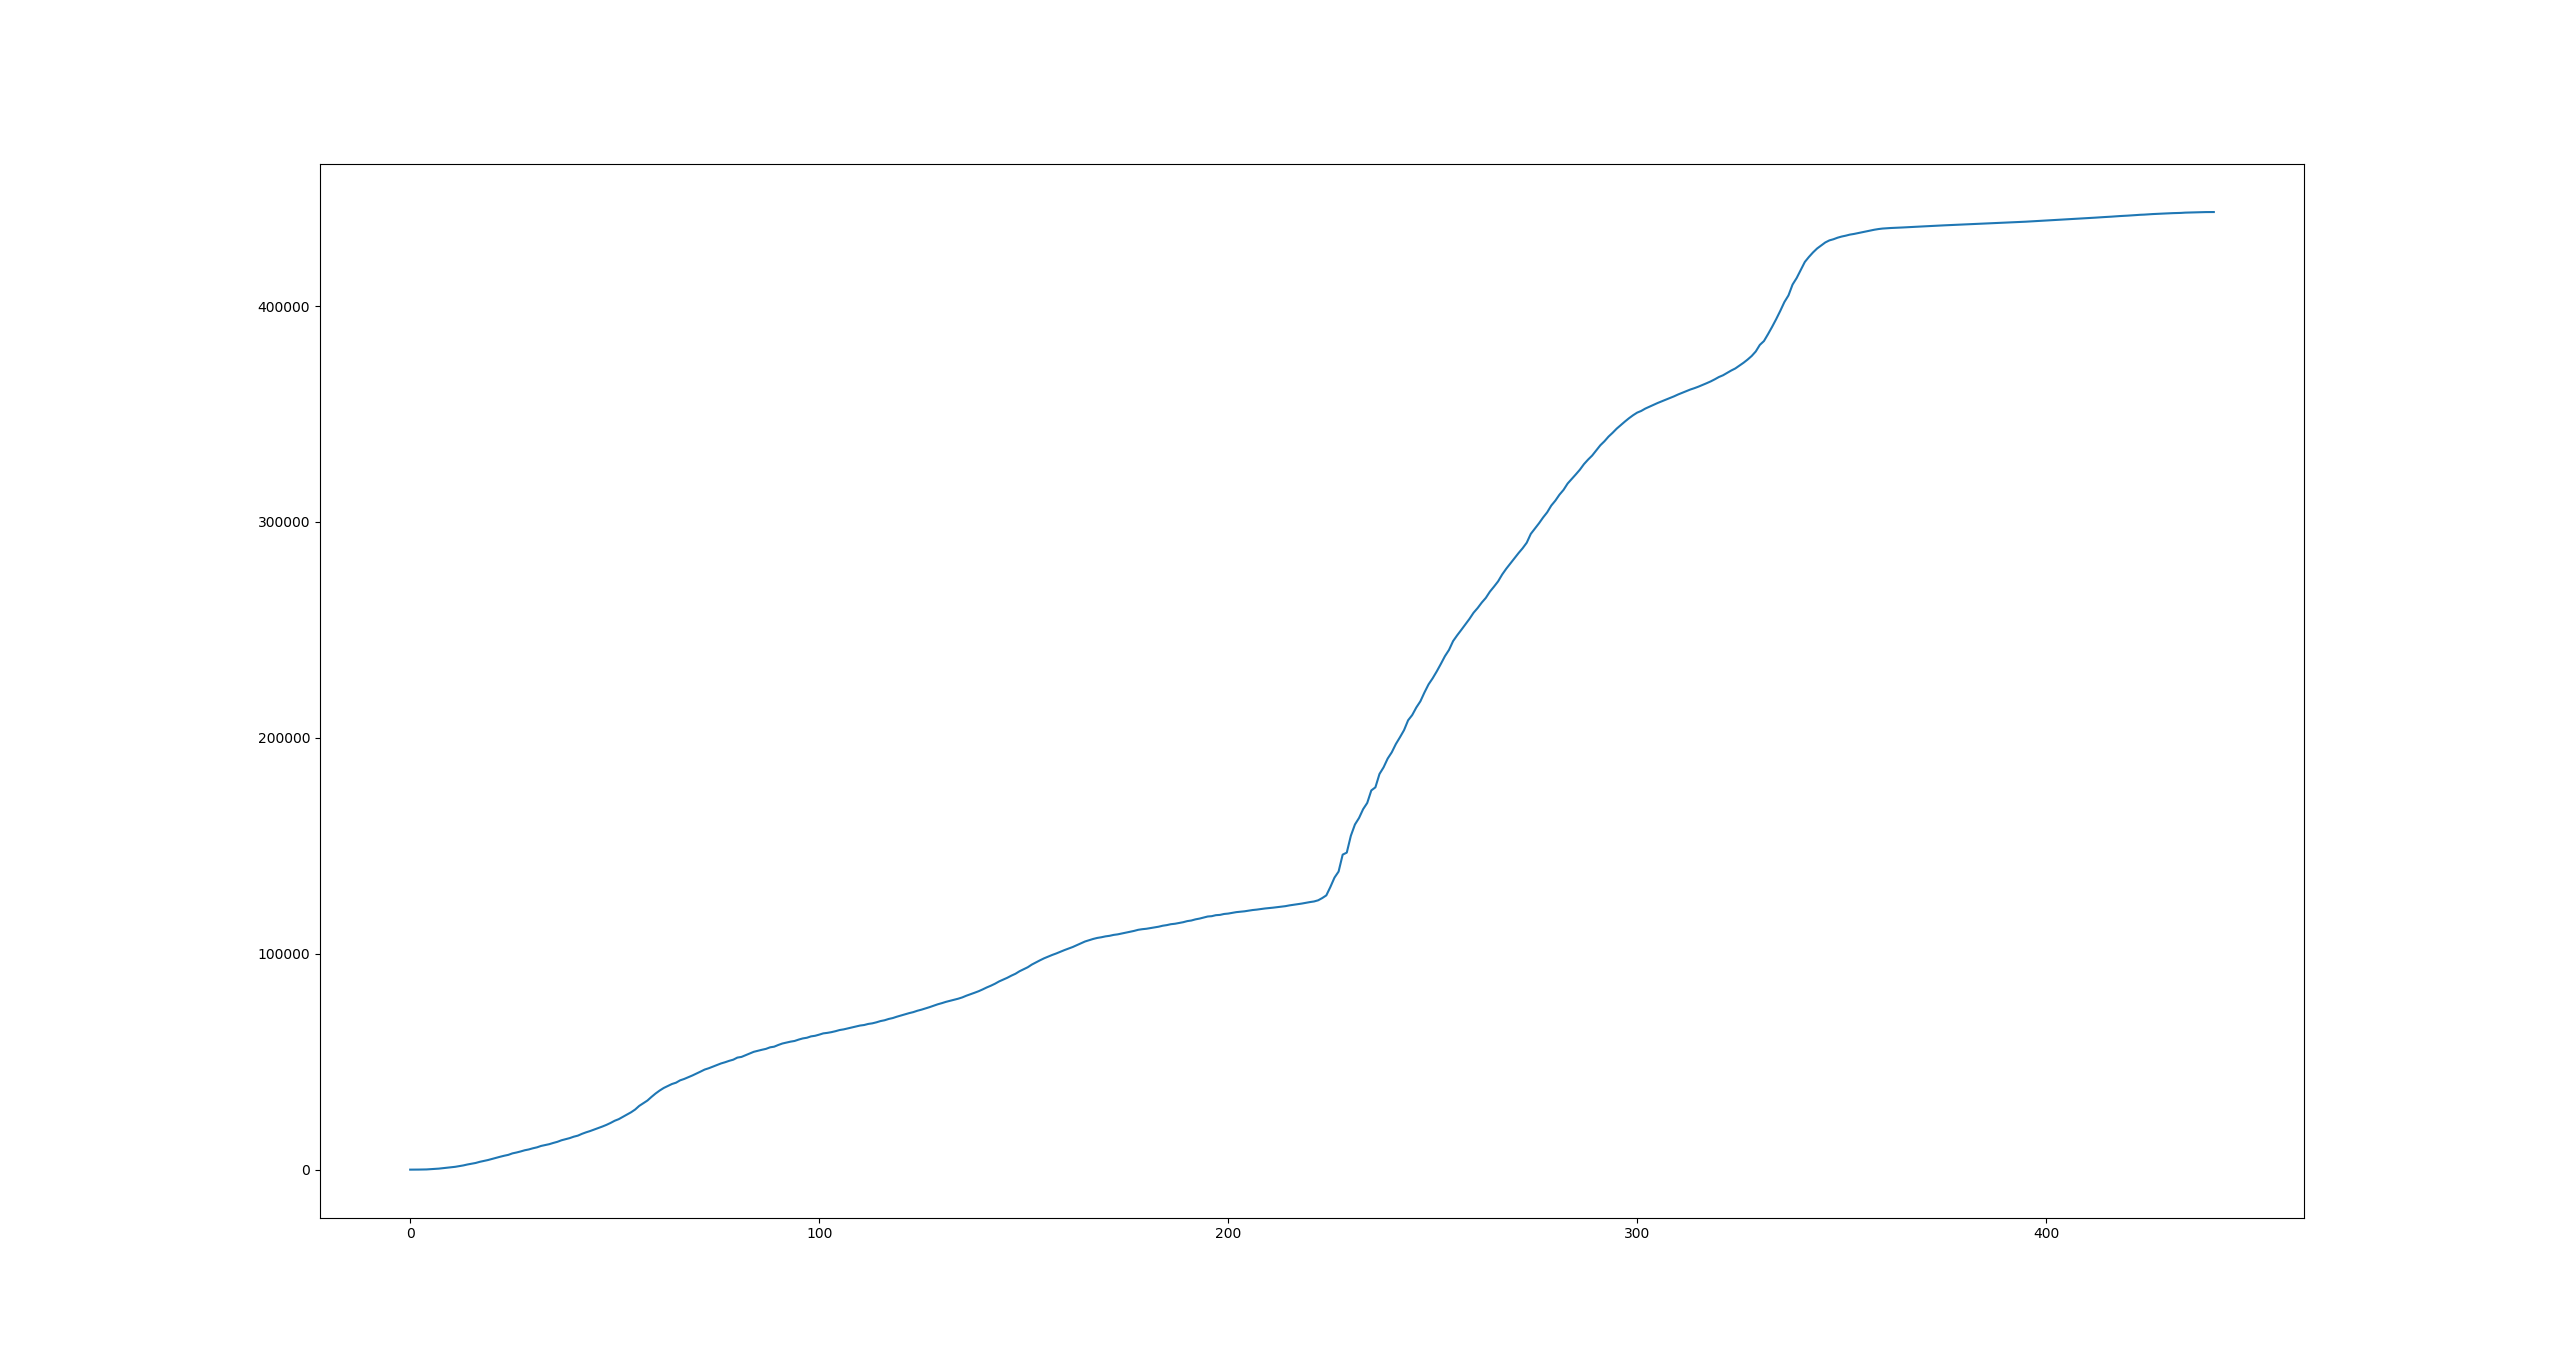
\includegraphics[scale=0.25]{pixels_per_radiu}
        \caption{Red}
    \end{figure}

    \begin{figure}[h]
        \centering
        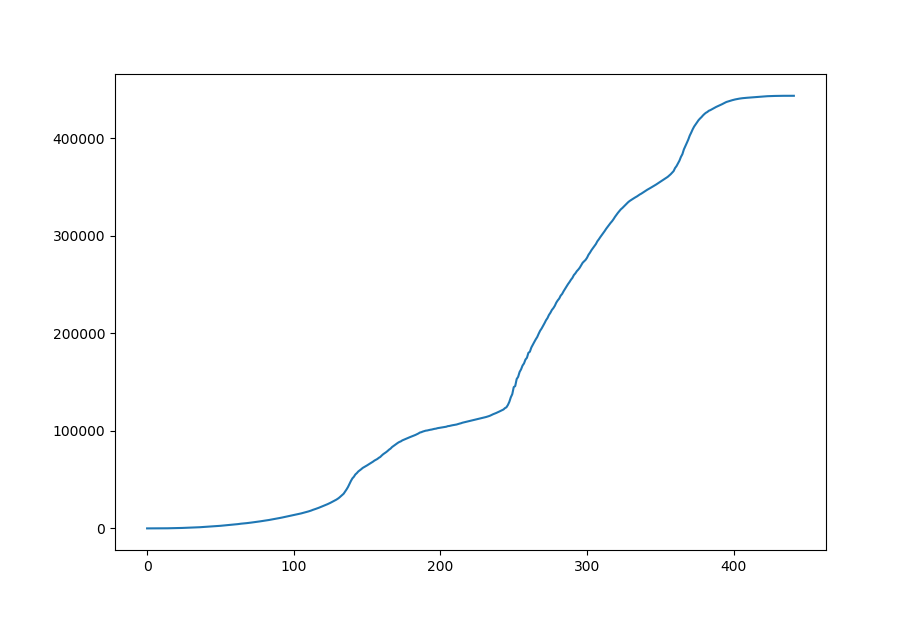
\includegraphics[scale=0.50]{pixels_per_radiu_green}
        \caption{Green}
    \end{figure}

    sos
    \subsection{Does it seem possible to select a good threshold value based on those curves?}
    Probably one of the places where the slope of the function changes radically is a good threshold.

    \subsection{With four different threshold radii, show the red and green binary masks that contain the segmented pixels}
        Used 45, 70, 90, 110

        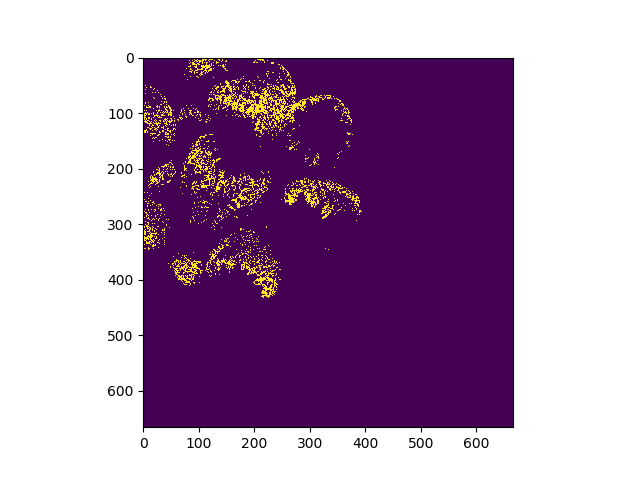
\includegraphics[height=50mm]{red_mask_45}
        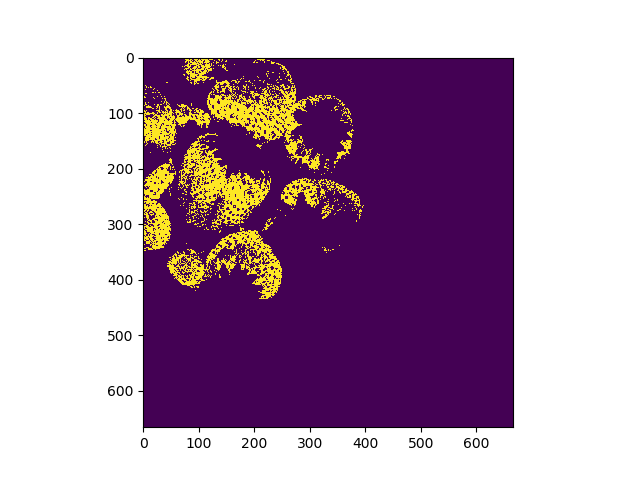
\includegraphics[height=50mm]{red_mask_70}
        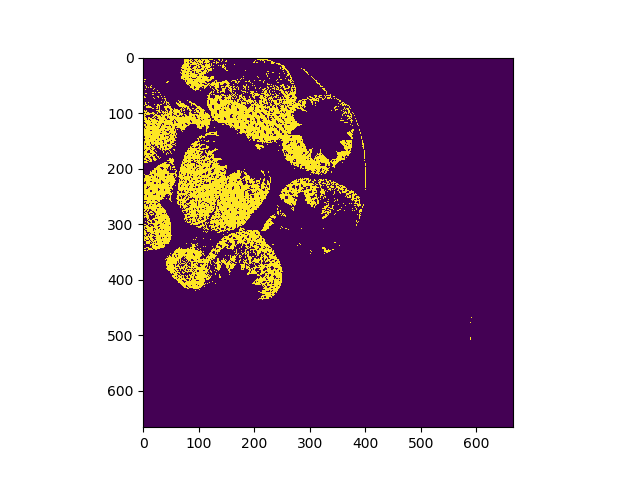
\includegraphics[height=50mm]{red_mask_90}
        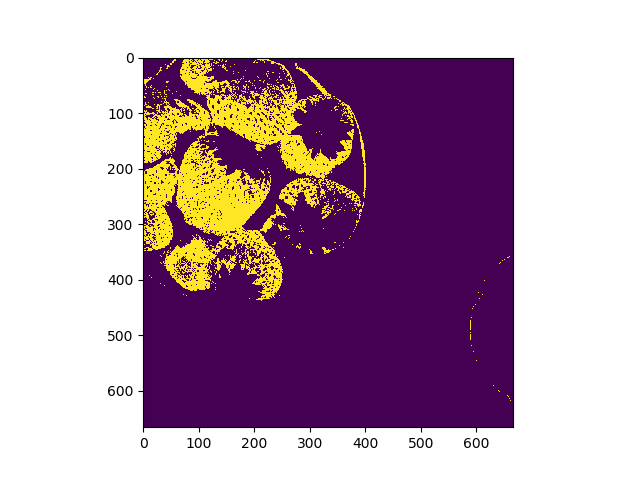
\includegraphics[height=50mm]{red_mask_110}

        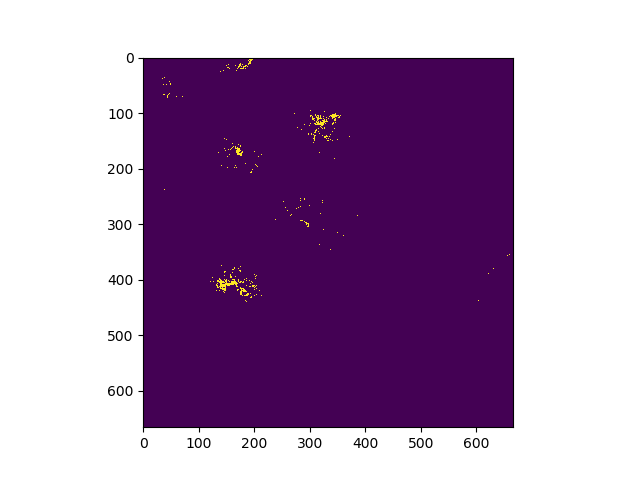
\includegraphics[height=50mm]{green_mask_45}
        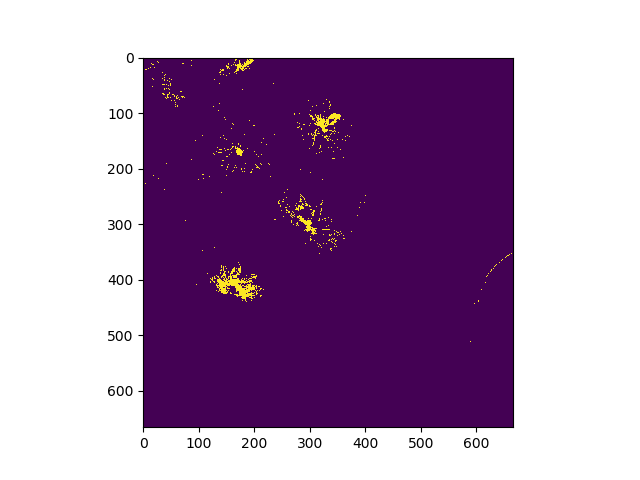
\includegraphics[height=50mm]{green_mask_70}
        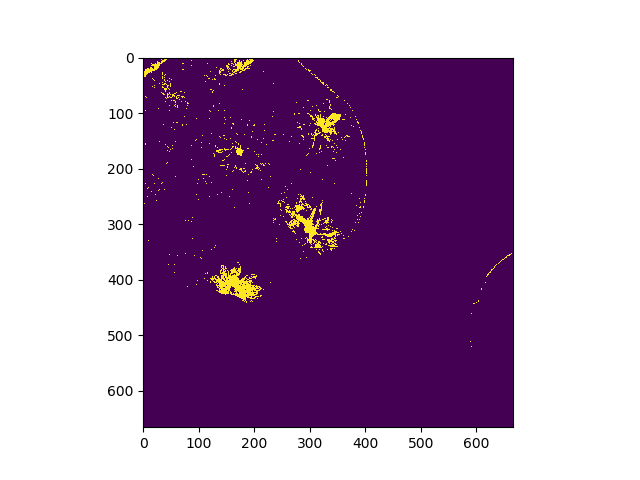
\includegraphics[height=50mm]{green_mask_90}
        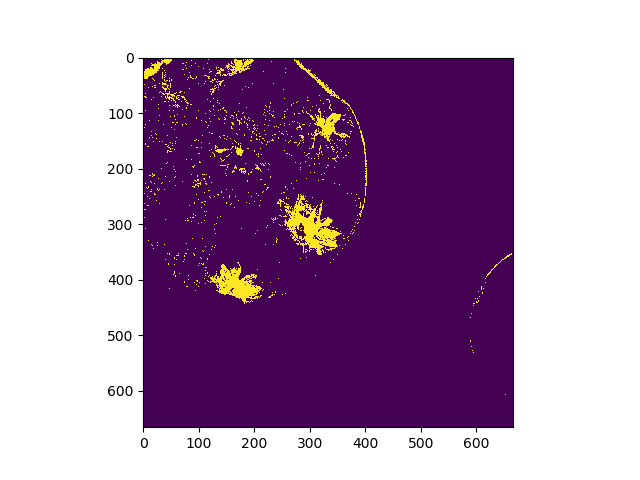
\includegraphics[height=50mm]{green_mask_110}
    \subsection{Select a good threshold radius that works for both read and green}
        90 seems to work alright for both.
    \subsection{Create a binary mask image of the segmented red and green pixels}
        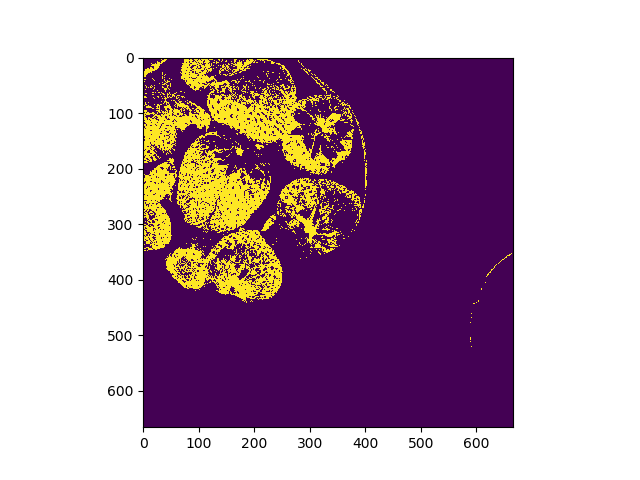
\includegraphics[height=100mm]{combined_red_green_90}

    \subsection{How long it took}
    Hands-on took 5 - 6 hours. 
    
    \noindent Homework took around 4 hours.

    \section{Homework code}
    \begin{verbatim}
### Task 1
# We will use image strawberries.tiff to study color-based segmentation and morphological closing
### Task 2?
# Select representative BGR sample points corresponding to the red and green colors in the berries
# wat?

import cv2
import numpy as np
import matplotlib.pyplot as plt
import matplotlib.cm as cm
from scipy import ndimage as nd
from scipy.spatial import distance

strawberries = cv2.imread('strawberries.tiff')
cv2.imwrite('strawberries.jpg', strawberries)

### Task 3
# Define spheres around the reference points and count how many pixels fall in them when increasing the radius from zero until all pixels are inside the spheres
def count_in_sphere(radius, distances):
    count = 0
    for column in distances:
        for distance in column:
            if(distance < radius):
                count += 1
    return count

def calc_distances(center, A):
    compare_color = A[center[0]][center[1]]
    distances = np.full((strawberries.shape[0], strawberries.shape[1]), 0)
    x, y = 0,0
    for column in A:
        for pixel in column:
            distances[y][x] = distance.euclidean(compare_color, pixel)
            x += 1
        x = 0
        y += 1
    return distances


#print('derp ' + str(count_in_sphere((65, 200), 10, strawberries)))
# strawberry red area
#cv2.imshow("red", cv2.resize(strawberries[30:100, 150:250], None, fx=2, fy=2, interpolation=cv2.INTER_AREA))


red_distances = calc_distances((65, 200), strawberries)

red_enabled = False
if red_enabled:
    pixel_count = strawberries.shape[0] * strawberries.shape[1]
    count = 0
    radius = 0
    count_per_radius_red = []
    while count < pixel_count and red_enabled:
        print('ratius ' + str(radius))
        radius += 1
        count = count_in_sphere(radius, red_distances)
        count_per_radius_red.append(count)

    print('doned')
    plt.plot(count_per_radius_red)
    plt.show()
    plt.savefig('pixels_per_radius_red.png')

# strawberry green area 
#cv2.imshow("green", cv2.resize(strawberries[100:180, 280:370], None, fx=2, fy=2, interpolation=cv2.INTER_AREA))
#cv2.waitKey()

green_distances = calc_distances((120, 300), strawberries)

green_enabled = False
if green_enabled:
    pixel_count = strawberries.shape[0] * strawberries.shape[1]
    count = 0
    radius = 0
    count_per_radius_green = []
    while count < pixel_count and green_enabled:
        print('ratius ' + str(radius))
        radius += 1
        count = count_in_sphere(radius, green_distances)
        count_per_radius_green.append(count)

    print('doned')
    plt.plot(count_per_radius_green)
    plt.show()
    plt.savefig('pixels_per_radius_green.png')


### Task 5
#Does it seem possible to select a good threshold value based on those curves?
#yes
### Task 6
# With four different threshold radii, show the red and green binary masks that contain the segmented pixels

def mark_pikkels(radius, distances):
    mask = np.full((distances.shape[0], distances.shape[1]), 0)
    for y in range(len(distances) - 1):
        for x in range(len(distances[y]) - 1):
            if(distances[y][x] < radius):
                mask[y][x] = 1
    return mask

green_mask_45 = mark_pikkels(45, green_distances) * 255
green_mask_70 = mark_pikkels(70, green_distances) * 255
green_mask_90 = mark_pikkels(90, green_distances) * 255
green_mask_110 = mark_pikkels(110, green_distances) * 255

plt.imshow(green_mask_45)
plt.savefig('green_mask_45.png')
plt.imshow(green_mask_70)
plt.savefig('green_mask_70.png')
plt.imshow(green_mask_90)
plt.savefig('green_mask_90.png')
plt.imshow(green_mask_110)
plt.savefig('green_mask_110.png')

red_mask_45 = mark_pikkels(45, red_distances) * 255
red_mask_70 = mark_pikkels(70, red_distances) * 255
red_mask_90 = mark_pikkels(90, red_distances) * 255
red_mask_110 = mark_pikkels(110, red_distances) * 255
plt.imshow(red_mask_45)
plt.savefig('red_mask_45.png')
plt.imshow(red_mask_70)
plt.savefig('red_mask_70.png')
plt.imshow(red_mask_90)
plt.savefig('red_mask_90.png')
plt.imshow(red_mask_110)
plt.savefig('red_mask_110.png')

### Task 7
# Select  a  good  threshold  radius  that  works  for  bothread and green90
# 90 seems to work alright for both

### Task 8
# Create a binary mask image of the segmented red and green pixels
def combine(red, green):
    combined = np.full((red.shape[0], red.shape[1]), 0)
    for y in range(len(red) - 1):
        for x in range(len(red[y]) - 1):
            if red[y][x] == 1 or green[y][x] == 1:
                combined[y][x] = 1
    return combined

combined = combine(red_mask_90/255, green_mask_90/255)

plt.imshow(combined * 255)
plt.savefig('combined_red_green_90.png')
    \end{verbatim}


\end{document}
%  LocalWords:  Jorma Laaksonen pdf py tex OpenCV libopencv dev jpg
%  LocalWords:  highgui imgproc imgcodecs greyscale png opencv ing
%  LocalWords:  texlive includegraphics Exactum Gür Ersalan
